\documentclass{book} 
\usepackage{graphicx} % Required for inserting images
\usepackage{mathrsfs}
\usepackage{amssymb}
\usepackage{amsmath}
\usepackage{indentfirst}
\usepackage{color}
\usepackage{hyperref}
\usepackage{xypic}
\usepackage{bbm}
\usepackage{xeCJK}
\usepackage{dutchcal}
\usepackage{pgfplots}
\usepackage{expl3}
\hypersetup{hidelinks,
	colorlinks=true,
	allcolors=black,
	pdfstartview=Fit,
	breaklinks=true
}
\newcommand{\abs}[1]{\left\lvert #1 \right\rvert} 
\newcommand{\norm}[1]{\left\lVert #1 \right\rVert}
\newcommand{\leftbracket}{[}
\newcommand{\rightbracket}{]}
\newcommand{\inprod}[2]{\left<#1,#2\right>}
\newcommand{\set}[1]{\left\{#1\right\}}
\newcommand{\fpart}[3][]{\frac{\partial^{#1}#2}{\partial #3^{#1}}}
% \newcommand{\mapping}[5][]{
% \ExplSyntaxOn
% \cs_if_exist:NTF {#1}
% {\begin{aligned}
%     #1:&#2&\rightarrow&#3\\ &#4&\mapsto&#5
% \end{aligned}}  
% {\begin{aligned}
%     &#2&\rightarrow&#3\\ &#4&\mapsto&#5
% \end{aligned}}
% \ExplSyntaxOff
% }
\begin{document}
\tableofcontents
\chapter{Preface}
\section{Ref}
\begin{itemize}
    \item Ahlfors: Complex analysis.
    \item 谭小江,伍胜健 复变函数简明教程
    \item Stein,? complex analysis.(extra exercises)
\end{itemize}
\section{A brief history of complex analysis}
Complex analysis refers studies on functions of complex variables, emerged in the 19th century. Cauchy proposed Cauchy 's integral theorem (1825) and the concept of residues. Riemann defined the Riemann Surface, which enlarge complex analysis to geometry field. Besides, he defined Riemann zeta function. And he gave Riemann mapping theorem. Weirstrass use power series to approach complex analysis.

Complex analysis also deeply connects to other filed in math.
\begin{itemize}
    \item It's essential to analysis geometry and complex geometry.
    \item Provide powerful tool to research prime numbers.
    \item In dynamics, complex dynamics is active.
    \item Deep connected with topology of 3-manifold.
    \item Deep connection with harmonic analysis(Fourier analysis).
\end{itemize}
\part{Review of learnt}
\chapter{Definition of complex numbers}
$\mathbb{R}$ denotes the real numbers. Some polynomials equation like $x^2+1=0$ has no solutions in $\mathbb{R}$. So we formally introduce the number $i$ (an imaginary number) s.t.$$i^1+1=0$$
A complex number $z=a+bi$, where $a,b\in \mathbb{R}$. Let $$\mathbb C=\{z=a+bi\mid a,b\in \mathbb R\}$$ 
$\mathbb C$ is called complex plane. The real numbers $a,b$ are called the real and imaginary part of $z$ respectively. Denoted by $\Re z,\ \Im z$

Similar with to $\mathbb R$, we can define a field structure on $\mathbb C$.\begin{itemize}
    \item[Addition]$$(a+bi)+(c+di)=(a+c)+(b+d)i$$
    \item[Multiplication]$$(a+bi)\cdot(c+di)=(ac-bd)+(ad+bc)i$$ 
\end{itemize}
To verify $\mathbb C$ a field, we need to show $\forall z\neq 0,\ \exists z^{-1}$
\section{Def: complex conjugation}Let $z\in \mathbb C$. The complex conjugation $\overline z$ of $z=a+bi$ is
$$\overline z=a-bi$$
Ones can verify are $$\overline{z+w}=\overline z+\overline w$$
$$\overline{zw}=\overline{z}\overline{w}$$
As a corollary, we consider a polynomial equation
$$a_nz^n+\cdots+a_0=0\quad a_i\in \mathbb{C}$$. If $z$ is a root, then $\overline z$ a root for:
$$\overline{a_n}z^n+\cdots+\overline{a_0}=0$$
In particular, $a_i\in\mathbb R$, then $\overline z$ is also a solution to original equation.
\section{Def:absolute value}
The absolute value of complex number $z$ is defined as:
$$\abs{z}:=\sqrt{z\cdot\overline z}=\sqrt{a^2+b^2}$$ one can verify:
$$\abs{zw}=\abs z\cdot\abs w$$
$$\abs{z+w}^2=\abs{z}^2+\abs{w}^2+2\Re(z\overline w)$$
$$\abs{z-w}^2=\abs{z}^2+\abs{w}^2-2\Re(z\overline w)$$
\section{Def: division}
Let $z_1,z_2\in \mathbb C$
$$\frac{z_1}{z_2}:=\frac{z_1\overline {z_2}}{\abs{z_2}^2}$$
In particular, if $z=a+bi$$$z^{-1}=\frac{\overline z}{\abs{z}^2}$$
\chapter{Geometry picture of complex numbers}
We can identify $\mathbb C\cong \mathbb R^2$ as $\mathbb R$-vector space, by using $z=a+bi$. We can also use the polar coordinates write $z=r(\cos\theta+i\sin\theta)$, where $r=\abs{z}$, $\theta$ is called the argument of $z$. Then conjugation flip $z$ along real axis. Addition is the same with vectors' addition. Multiplication multiplicate the length of vector and rotate the vector by the other's argument.

Consider the equation $z^n=1, \ n\geq 1$. The solution of it is called $n$-th root of unity.

\section{Some inequalities}
By the definition of absolute value
$$-\abs z\leq\Re z\leq\abs z$$
$$-\abs z\leq\Im z\leq\abs z$$
The equality $\Re z=\abs z$ iff $z$ is a non-negative real number. Since $Re(z\overline{w})\leq\abs z\abs w$ recall for $z,w \in \mathbb C$$$\abs{z+w}^2=\abs z^2+\abs w^2+2\Re(z\overline w)$$
Then we get triangle inequality:
$$\abs{z+w}\leq\abs z+\abs w$$
\subsection{Cauchy's inequality}
Let $n\geq 1$, then $$\abs{\sum\limits_{k=1}^nz_kw_k}^2\leq(\sum\limits_{k=1}^n\abs {z_k}^2)(\sum\limits_{k=1}^n\abs {w_k}^2)$$ with the equality holds iff $\exists t\in \mathbb C, \forall 1\leq k\leq n, z_k+t\overline{w_k}=0$
\subsubsection*{Proof}
Let $t\in \mathbb C$ be any complex number
$$\begin{aligned}
    0 &\leq\sum\limits_{k=1}^n\abs{z_k+t\overline {w_k}}^2=\sum\limits_{k=1}^n\abs{z_k}^2+\abs{t}^2\sum\limits_{k=1}^n\abs{w_k}^2+2\Re(\overline t\sum\limits_{k=1}^n z_kw_k)
\end{aligned}$$
choose $t=\frac{\sum\limits_{k=1}^nz_kw_k}{\sum\limits_{k=1}^n\abs{w_k}^2}$
Then we get
$$\sum\limits_{k=1}^n\abs{z_k}^2=\frac{\abs{\sum\limits_{k=1}^nz_kw_k}^2}{\sum\limits_{k=1}^n\abs{w_k}^2}\geq 0$$
The condition of equality $\Leftarrow$ the equality $0=\sum\limits_{k=1}^n\abs{z_k+t\overline {w_k}}$
\chapter{Topology and metrics on $\mathbb C$}
\section{Basic definitions}
Recall that a topology space is a set $X$ equipped with a collection of subsets of $X$ as open sets, satisfying:
\begin{itemize}
    \item $X$ and $\varnothing$ are open.
    \item Arbitrary union of open sets is open
    \item Finite intersection of open sets is open.
\end{itemize}
A closed set is by definition the complement of an open set.

A metric space is a pair $(X,d)$, where $X$ be a set and $d:X^2\rightarrow \mathbb{R}_{\geq 0}$ a mapping s.t.
\begin{itemize}
    \item $d(x,x)=0\quad\forall x\in X$
    \item $d(x,y)>0\quad\forall x\neq y\in X$
    \item $d(x,y)=d(y,x)$
    \item $d(x,y)\leq d(x,z)+d(z,y)$
\end{itemize}
let $x\in X, r>0\in \mathbb R$ the set $$\mathcal B(x,r):=\{y\in X\mid d(x,y)<r\}$$ is called an open ball. We say a subset $N\subseteq X$ is a neighborhood of $x$ if N contains an open ball centered at $x$. A subset N is open if $\forall x\in N$ N is a neighborhood of $x$
\subsection*{Remark}
For any subset $N\subseteq X$ $(N,d)$ is a metric space. The diameter of $X$:$$diam X:=\sup\limits_{x,y\in X}d(x,y)$$
X is bounded if $diam X<+\infty$. A sequence of points $x_n$ in X is called converges to $x\in X$ if $\lim\limits_n\rightarrow+\infty d(x_n,x)=0$. A sequence $(x_n)$ is called Cauchy sequence if $\forall \epsilon>0,\exists N\geq1$ s.t. $\forall n>m\geq N, d(x_n,x_m)<\epsilon$

The metric space is called complete if any Cauchy sequence converges.
\section{Notations}
$N\subseteq X$ any subset.
\begin{itemize}
    \item $\mathring N$ the interior of N, is the maximal open subset contained in N, i.e. $$\mathring N=\text{ union of all open subsets in N}$$
    \item $\overline N$ the \textbf{closure} of $N$, the minimal closed set contains $N$.
    \item $\partial N$ the \textbf{boundary} of $N$, $$\partial:=\overline N\setminus \mathring N$$let $N\subseteq X$. A point $x\in X$ is a limit point of $N$ if $x\in \overline N$ $\Leftrightarrow$ this means $\exists$ sequence $(x_n)$ in N s.t. $x_n\rightarrow x$ ($\lim\limits_{n\rightarrow+\infty}d(x_n,x)=0$)
    \item We say $x\in X$ is called an \textbf{isolated} point if $\exists$ an open ball $\mathcal B(x,r)$ s.t. $$\mathcal B(x,r)\cap X=\{x\}$$
    \item We say X is \textbf{connected} if X is not a disjoint union of non-empty open subsets.
    \item a point $x\in X$ is called a \textbf{limit point} of $N$ if $x\in \overline N$ $\Leftrightarrow$ this means $\exists$ sequence $(x_n)$ in N s.t. $x_n\rightarrow x$ ($\lim\limits_{n\rightarrow+\infty}d(x_n,x)=0$)
\end{itemize}
\chapter{Compactness}
An open cover of $X$ is a collection of open sets $\{U_\alpha\}$, $X=\bigcup\limits_\alpha U_\alpha$

X is called totally bounded if $\forall \epsilon>0, \exists$ finite open cover using $\epsilon-$radius balls. It's clear that totally bounded set is bounded.

The metric space X is called compact if every open cover of X has a finite sub-cover.
\section{Theorem}
A metric space X is compact $\Leftrightarrow$ X is complete and totally bounded.
\subsection*{Proof}
\subsubsection{$\Rightarrow$}
For completeness, assuming X isn't. Then exists a Cauchy sequence $(x_n)$ doesn't converges. Then $\forall y\in X, x_n\not\rightarrow y$. Then $\exists r>0$ s.t. $\cup_y:=\mathcal{B}(y,r)$ then $\cup_y$ contains finite many elements. Then we get an open cover $\{\cup_y\}_{y\in X}$. For X compact, we can get a finite subcover.$$X=\bigcup\limits_{y\in F}\cup_y$$where F finite.In particular $x_n\in \bigcup\limits_{y\in F}\cup_y$ so $X_n=\{x_n\mid n\in \mathbb N\}$ contains finite many elements. But finite Cauchy sequence converges. Contradiction.

For total boundence. For every $\epsilon>0, y\in X$ let $\cup_y:=\mathcal{B}(y,\epsilon)$ Then $\{\cup_y\}_{y\in X}$ is an open cover. For compactness, we get a finite subcover $X\subseteq\bigcap\limits_{y\in F}\cup_y$ so X totally bounded.
\subsubsection{$\Leftarrow$}Assume X is complete and totally bounded Assume X is not compact. Then $\exists$ open cover $\{U_\alpha\}$ s.t. $
\not\exists$ finite subcover. For totally bounded, $X=\bigcap\limits_{x\in F}\mathcal{B}(x,1)$ F finite. Then consider the index in F s.t. $\mathcal{B}(x,1)\neq\bigcup\limits_{\alpha\in E}\cup_\alpha\cap\mathcal B(x,1)$ Then exist $x_0$ s.t. $\mathcal B(x_0,1)$ can not be covered by finite many $\cup_\alpha$ So $\exists x_1\in \mathcal{B}(x_0,1)$ s.t. $\mathcal B(x_1,2^{-1})$ cannot be covered by finite many $\cup_\alpha$. Inductively, we get a sequence $(x_n)_{n\in \mathbb N}$. $$d(x_n,x_{n+1})\leq 2^{-n}$$ which means $(x_n)$ is Cauchy sequence. Moreover, $\mathcal B(x_n,2^{-n})$ can't be covered by finite many $\cup_\alpha$. By completeness, $(x_n)\rightarrow y\in X$ Let $U$ be an open set s.t. $U\in \{U_\alpha\}$ and $y\in U$. Then for $n$ large$$\mathcal B(x_n,2^{-n})\subseteq U$$contradiction.
\section{Theorem}A metric space X. Compact is equiv with Cauchy compact.
\subsection*{Proof}
\subsubsection{$\Leftarrow$}
Assume X Cauchy compact. We prove it by prove X complete and totally bounded. 

For a Cauchy sequence $(x_n)_{n\in \mathbb N}$ converges iff $\exists$ subsequence $(x_{n_i})$ converges. This means every sequence in X converges, meaning X complete.

Assume X isn't totally bounded. Then $\exists \epsilon>0$ s.t. X isn't covered by finite $\epsilon$-balls. We inductively construct a sequence $(x_n)$ as following: We choose $x_{n+1}$ s.t. $x_{n+1}\not\in \bigcup\limits_{k=1}^n\mathcal B(x_k,\epsilon)$ It doesn't have a subsequence convergent. Contradiction.
\subsubsection{$\Rightarrow$}
Assume that $\exists(x_n)_{n\in \mathbb N}$ divergent. Then $\forall y\in X,\exists r>0$ s.t. $$\cup_y:=\mathcal B(y,r)$$
$\cup_y$ contains finite points in $\{x_n\}$. Then consider the open cover $\{\cap_y\}_{y\in X}$. According to compactness, extract a finite sub-cover: $X\subseteq\bigcup\limits_{y\in F}\cup_y$. Then $\{x_n\}$ a finite set, which means $(x_n)$ has a convergent subsequence. For Cauchy sequence this implies convergence. Contradiction.
\section{Def}
Consider $X=\mathbb C$ $\forall z,w\in \mathbb C$ $$d(z,w):=\abs{z-w}$$ open balls in $\mathbb C$ is called open disks $\mathcal D(z,r)$ $$\mathbb D:=D(0,1)$$ is called unit disk.
\section{Lemma}A sequence $z_n\rightarrow z$ in $\mathbb C$$\Leftrightarrow$ \begin{itemize}
    \item $\Re z_n\rightarrow\Re z$
    \item $\Im z_n\rightarrow =\Im z$
\end{itemize}
\section{Theorem} $\mathbb C$ is complete.
\subsection*{Proof}This follows $\mathbb R$ is complete and the Lemma above.
\section{Lemma} A bounded subset in $\mathbb C$ is totally bounded.
\subsection*{Proof}
Let $K\subseteq\mathbb C$ bounded. $\exists R>0$ s.t. $K\subseteq \mathcal{D}(0,R)$. It suffice to show $\mathcal D(0,R)$ is totally bounded. It's clear, since $\mathcal{D}(0,R)$ can be covered by finitely many $\epsilon-$balls.
\section{Corollary}
A subset $K\subseteq \mathbb C$ is compact $\Leftrightarrow$ K is bounded and K is closed. 
\subsection*{Proof}K is compact $\Leftrightarrow$ K is totally bounded and complete. Since $\mathbb C$ complete, K is complete iff K is closed. Then $K$ compact $\Leftrightarrow$  K closed and bounded.
\section{Continuous mapping}
$f:X\rightarrow Y$ between metric space is continuous if $\forall$ open set $U\subseteq Y\ f^{-1}(U)$ is open

A homomorphism $f:X\rightarrow Y$ continuous and $f^{-1}$ is also continuous.
\section{Lemma}
Let $f:X\rightarrow Y$ between metric space $f$ is continuous $\Leftrightarrow$ $\forall$ sequence $(x_n)$ in X $x_n\rightarrow x\Rightarrow f(x_n)\rightarrow f(x)$
\section{Theorem}
$f:X\rightarrow Y$ continuous mapping between metric spaces. Let $K\subseteq X$ compact. Then $f(K)$ is compact in Y.
\subsection*{Proof}
Any open cover $\{V_\alpha\}$ of $f(K)$ induces an open cover $U_\alpha:=f^{-1}V_\alpha$ of K. Since K is compact, $\exists$ finite set $F$ s.t. $$K=\bigcup\limits_{\alpha\in F}U_\alpha$$
then $$f(K)=\bigcup\limits_{\alpha\in F}V_\alpha$$
so $f(K)$ is compact.
\section{Corollary}
Let X compact metric space. Let $f:X\rightarrow \mathbb R$ continuous function. Then $f(X)$ can take maximal and minimal values.
\subsection*{Proof}
$f(x)$ is compact in $\mathbb R$
\section{Theorem}$f:X\rightarrow Y$ continuous. If X is connected, then $f(X)$ is connected.
\subsection{Proof}
Assume that $f(X)=A\cup B$, with A, B non-empty and disjoint. Then $X=f^{-1}(A)\cup f^{-1}(B)$ is a union of non-empty open sets, meaning X not connected.
\section{Def}
Let $f:X\rightarrow Y$ continuous mapping $f$ is called uniformly continuous if $\forall \epsilon>0,\exists \delta>0$ s.t. if $d(x,y)<\delta$, then $d(f(x),f(y))<\epsilon$.
\section{Theorem}Let $f:X\rightarrow Y$ continuous. X compact. Then $f$ uniformly continuous.
\chapter{Path connected and homotopy}
A curve in $\mathbb C$ is a continuous mapping $\gamma:[a,b]\rightarrow \mathbb C$
\section{Def}
A subseteq $S\subseteq \mathbb C$ is called path-connected if $\forall z,w\in S,\exists \gamma:[a,b]\rightarrow S$ curve s.t. $\gamma(a)=z,\gamma(b)=w$
\section{Theorem}Let $U\subseteq \mathbb C$ open set. $U$ is connected $\Leftrightarrow$ path connected.
\subsection*{Proof}
Let $U\subseteq \mathbb C$ open $\forall z\in U$ let $$V_z:=\{\text{points} w\in U\text{ s.t.}\exists\text{curve connecting }z,w\}$$
Since every open disk is path connected, $V_z$ is open, $U\setminus V_z$ is open.
\subsubsection{$\Rightarrow$}
Assume U not path connected. Then $\exists z\in U$ s.t. $V_z\neq U$. Let $V_1:=V_z, V_2:=U\setminus V_z$. Then $V_1,V_2$ are non-empty open disjoint sets, then U not connected. Contradiction.
\subsubsection{$\Leftarrow$}
Assume U not connected. We can write $$U=V_1\cup V_2$$$V_1,V_2$ non-empty and disjoint open sets. Let $z\in V_1,w\in V_2$ and $\gamma:[a,b]\rightarrow U$ curve $\gamma(a)=z,\gamma(b)=w$. Let $$I_1:=\gamma^{-1}V_1\quad I_2:=\gamma^{-1}V_2$$ $I_1,I_2$ open non-empty and disjoint and $[a,b]\cup I_1,I_2$, telling $[a,b]$ not connected. Contradiction.


\subsection{Remark}This conclusion isn't true in general when U is not open. Consider $$S:\{i y\mid\abs y\leq 1\}\cup\{x+i\sin\frac{1}x\mid 0<x\leq 1\}$$
S closed. Try to prove:\begin{itemize}
    \item S connected
    \item S not path connected
\end{itemize}
\section{Def:homotopy}
Let $U\subseteq \mathbb C$ be an open set. Let $\gamma_0:[a,b]\rightarrow U$, $\gamma_1:[a,b]$ be two curves. A homotopy between $\gamma_0$ and $\gamma_1$ is a continuous mapping $$H:[0,1]\times[a,b]\rightarrow U$$ s.t. $$H(0,t)=\gamma_0(t)\quad H(1,t)=\gamma_1(t)$$
and $\forall s\in [0,1]$
$$H(s,a)=\gamma_0(a)\quad H(s,b)=\gamma_0(b)$$
We call $\gamma_0,\gamma_1$ are homotopic if $\exists$ such a mapping.
\section{Def}
Let $U\subseteq \mathbb C$ be a connected open set. U is called simply connected if $\forall$ two curves in U with same starting and end pts are homotopic.
\chapter{Complex value function and holomorphic function}
\section{Def:Complex valued function}
$U\subseteq \mathbb C$ a open set. \textbf{Complex value function} is a mapping $f:U\rightarrow \mathbb C$ We can view $$f=u(x,y)+i(x,y)$$ via $\mathbb C\cong\mathbb R^2, z=x+iy$. We say that $f$ is differentiable if $u,v$ are differentiable. In particular, $\exists$ partial derivatives $$\frac{\partial u}{\partial x},\frac{\partial u}{\partial y},\frac{\partial v}{\partial x},\frac{\partial v}{\partial y}$$
For $z=x+iy\in U$, define:
$$\frac{\partial f}{\partial x}(z):=\frac{\partial u}{\partial x}(z)+i\frac{\partial v}{\partial x}(z)$$
\section{Def: Differential form}
Let $U\subseteq \mathbb C$ open. A differential form is a formal sum $g\text{d}x+h+\text{d}y$, where $g,h:U\rightarrow \mathbb C$ complex valued function.

Let $f:U\rightarrow \mathbb C$ differentiable. Define $$\text{d}f:=\frac{\partial f}{\partial x}\text{d}x+\frac{\partial f}{\partial y}\text{d}y$$
\section{Prop}
Let $f,g:U\rightarrow \mathbb C$ differentiable
\begin{itemize}
    \item[Linearity] $$\text{d}(f+g)=g\text{d}f+f\text{d}g$$
    \item[Leibniz rule]$$\text{d}(fg)=\text{d}f g+g\text{d}f$$ 
\end{itemize}

$z:\mathbb C\rightarrow\mathbb C,\overline z:\mathbb C\rightarrow \mathbb C$, then 
$$\text{d}z=\text{d}x+i\text{d}y,\text{d}\overline z=\text{d}x-i\text{d}y$$
$\Rightarrow$$$\text{d}x=\frac{1}2(\text{d}z+\text{d}\overline z)\quad \text{d}y=\frac{1}{2i}(\text{d}z-\text{d}\overline z)$$
$\Rightarrow$$$\text{d}f=\frac{1}2(\frac{\partial f}{\partial x}-i\frac{\partial f}{\partial y})\text{d}z+\frac{1}2(\frac{\partial f}{\partial x}+i\frac{\partial f}{\partial y})\text{d}\overline z$$
This motivates $$\partial f:=\frac{\partial f}{\partial z}\text{d}z$$
$$\frac{\partial f}{\partial z}:=\frac{1}2(\frac{\partial f}{\partial x}-i\frac{\partial f}{\partial y})$$
Similarly$$\overline{\partial f}:=\frac{\partial f}{\partial\overline z}\text{d}\overline z$$
$$\frac{\partial f}{\partial\overline z}:=\frac{1}2(\frac{\partial f}{\partial x}+i\frac{\partial f}{\partial y})$$
\section{Def:Holomorphic functions}
Let $U\subseteq \mathbb C$ open $f:U\rightarrow \mathbb C$. Let $z\in U$ we say $f$ is complex differentiable at $z$ if$$\lim\limits_{u\rightarrow z}\frac{f(u)-f(z)}{u-z}=f'(z)$$exists.

Geometrically: in the tangent space level, $f$ acts not just like a $\mathbb R$-linear mapping, but also a $\mathbb C$-linear mapping.

If $f:\mathbb R^2\rightarrow\mathbb R^2$ is $\mathbb R$-linear, then $f$ is complex differentiable iff $\exists a\in \mathbb C$, s.t.$$f(z)=az$$
\section{Def}
Let $U\subseteq \mathbb C$ open. $f:U\rightarrow \mathbb C$ is called holomorphic if $f$ is complex differentiable at every point in U.
\section{Lemma}
$U\subseteq \mathbb C$ open. $z\in U$, $f:U\rightarrow \mathbb C$, THen $f$ is complex differentiable at $z$ iff $f$ is real differentiable and satisfies the following Cauchy-Riemann equations:$$\frac{\partial f}{\partial \overline z}(z)=0$$
\subsection*{Proof}
\subsubsection{$\Leftarrow$} We can write $f(w)-f(z)=A(w-z)_o(\abs{w-z})$, where A is a real $2\times 2$ matrix. In the coordinate $z=x+iy,f=u+iv$$$A=\begin{pmatrix}
    \frac{\partial u}{\partial x}(z)&\frac{\partial u}{\partial y}(z)\\
    \frac{\partial v}{\partial x}(z)&\frac{\partial v}{\partial y}(z)
\end{pmatrix}$$
C-R equation:
$$\frac{\partial f}{\partial \overline z}\Leftrightarrow\begin{cases}
    \frac{\partial u}{\partial x}(z)&=\frac{\partial v}{\partial y}(z)\\
    \frac{\partial u}{\partial y}(z)&=-\frac{\partial v}{\partial x}(z)
\end{cases}$$
Define $$b:=\frac{\partial u}{\partial x}(z)=\frac{\partial v}{\partial y}(z)\in \mathbb R$$
$$c:=-\frac{\partial u}{\partial y}(z)=\frac{\partial v}{\partial x}(z)\in \mathbb R$$
Let $a:=b+ci\in \mathbb C$, then $$A(z)=az$$we can write$$f(u)-f(z)=a(w-z)+o(\abs{w-z})$$$\Rightarrow$ $f'(z)$exists.
\subsubsection{$\Rightarrow$}Trivial.
\section{Corollary}
$U\subseteq \mathbb C$ open set. $f:U\rightarrow \mathbb C$ $f$ is holomorphic on U iff $f$ is real differentiable on U and the C-R equation $$\frac{\partial f}{\partial \overline z}(z)=0\quad\text{holds }\forall z\in U$$
\chapter{Conformal matrix}
Let $A\in M_{2\times 2}(\mathbb R)$ be a matrix. $A:\mathbb R^2\rightarrow \mathbb R^2$ linear mapping. The inner product $v=(x_1,y_2),w=(x_2,y_2)$$$\inprod{v}{w}:=x_1x_2+y_1y_2$$$z,w\in \mathbb C$$$\inprod{z}{w}=\Re(z\overline w)$$

Let $J:\mathbb R^2\rightarrow\mathbb R^2, z\mapsto \overline z$ be the complex conjugation matrix. $\forall z,w\in \mathbb C$$$\inprod{Jz}{Jw}=\inprod{z}w$$
reflexction w.r.t. real axis.
\section{Def}A is called a rotation matrix if $$A=\begin{pmatrix}
    \cos\theta &-\sin\theta\\\sin\theta&\cos\theta
\end{pmatrix}$$
($\Leftrightarrow$ A present inner product and $\det A>0$)
\section{Prop}
A matrix A is given by $z\mapsto az,a\in \mathbb C$ $\Leftrightarrow$ $\exists\rho\geq 0$ and a rotation matrix $R_\theta$ s.t. $A=\rho R_\theta$$$\begin{cases}
    \rho=\abs{a}\\\theta=\arg z
\end{cases}$$
\section{Polar decomposition}
Any $A\in M_{2\times 2}(\mathbb R)$ can be written as $$A= R_\theta P$$or $$A=JR_\theta P$$, where $R_\theta$ is a rotation matrix, P is positive, semi-definite matrix.
\section{Def}
$A\in M_{2\times 2}(\mathbb R)$ is called conformal if A preserves the angle between two vectors i.e. $\forall z,w\in \mathbb C$$$\frac{\inprod{Az}{Aw}}{\abs{Az}\abs{Aw}}=\frac{\inprod{z}w}{\abs{z}\abs{w}} $$
\section{Remark}Conformal matrix is invertible. A circle in $\mathbb C$ is given by $$\{z\in \mathbb C\mid \abs{z-z_0}=r\}\quad r>0,z_0\in \mathbb C$$
\section{Prop}Let $A\in M_{2\times 2}(\mathbb R)$ s.t. $\det A>0$

(such matrix are called orientation preserving)

Then the following conditions are equivalent:
\begin{itemize}
    \item [1]A is conformal
    \item [2]A is given by $z\mapsto az, a\in C$
    \item [3]A maps a circle to a circle
\end{itemize}
\subsection*{Proof}
Since $\det A>0$ by polar decomposition$$A=\begin{cases}
    R_\theta P\\JR_\theta P
\end{cases}\Rightarrow A=R_\theta P$$
$R_\theta$ rotation, P positive semi-definite.

It suffices to prove the prop for P.
$$P=R_\beta DR_\beta^{-1}$$ where $D=\begin{pmatrix}
    \lambda_1&\\ &\lambda_2
\end{pmatrix},\lambda_1,\lambda_2>0$, and $R_\beta$ rotation.

It suffice to prove the prop for D. In this case (2)$\Leftrightarrow\lambda_1=\lambda_2$ It suffices to show (1)$\Rightarrow \lambda_1=\lambda$ and (3)$\Rightarrow\lambda_1=\lambda_2$

We first show (1)$\Rightarrow\lambda_1=\lambda_2$:

$D(1)=\lambda_1,D(1+i)=\lambda_1+\lambda_2i$, $$D=\begin{pmatrix}
    \lambda_1&\\ &\lambda_2
\end{pmatrix}$$. D conformal $\Rightarrow$ $$\frac{\inprod{Dz}{Dw}}{\abs{Dz}\abs{Dw}}=\frac{\inprod{z}{w}}{\abs{z}\abs{w}}$$
Take $z=1,w=1+i$
$$\frac{\inprod{\lambda_1}{\lambda_1+\lambda_2i}}{\lambda_1\sqrt{\lambda_1^2+\lambda_2^2}}=\frac{1,1+i}{\sqrt{2}}$$
Hence
$$\frac{\lambda_1^2}{\lambda_1\sqrt{\lambda_1^2+\lambda_2^2}}=\frac{1}{\sqrt 2}$$$\Rightarrow\ \lambda_1=\lambda_2$

Next (3)$\Rightarrow\ \lambda_1=\lambda_2$. Assume D maps circle to circle. Consider $\partial D(0,\sqrt 2)$. Then the image of $\partial D(0,\sqrt 2)$ is a circle, which is central symmetry w.r.t. $D(0)=0$. So the image is a circle centred at 0. Consider pts $\sqrt 2,1+i\in \partial D(0,\sqrt 2)$. Since $$D(\sqrt 2)=\lambda_1\sqrt 2\quad D(1+i)=\lambda_1+\lambda_2i$$ we have $$\abs{\lambda_1\sqrt 2}=\abs{\lambda_1+\lambda_2i}$$
$\Rightarrow \lambda_1=\lambda_2$
\chapter{Power series}
Let $n\in \mathbb Z$ one can verify
$$\begin{aligned}
    z^n:&\mathbb C&\rightarrow&\mathbb C\\ &z&\mapsto&z^n
\end{aligned}\quad n\geq0$$
$$\begin{aligned}
    z^{-n}:&\mathbb C\setminus\{0\}&\rightarrow&\mathbb C\\ &z&\mapsto&z^{-n}
\end{aligned}\quad n\geq0$$
we have
$$\frac{\partial z^n}{\partial z}=nz^{n-1}\quad\frac{\partial z^n}{\partial\overline z}=0$$
$$\frac{\partial \overline z^{-n}}{\partial z}=0\quad\frac{\partial \overline z^n}{\partial\overline z}=nz^{n-1}$$
so $z^n$ holomorphic but $\overline z$ not holomorphic.

In following we fix $n\in \mathbb Z$, $z^n:\mathbb C\rightarrow \mathbb C$, differentiable
\section{Def}
Let $z_0\in \mathbb C$ A \textbf{power series} centered at $z_0$ is of the form $$S=\sum\limits_{n=0}^{+\infty}a_n(z-z_0)^n\quad a_n\in \mathbb C$$
Let $z\in \mathbb C$. We say that S converges at $z$ if the number series $\sum\limits_{n=0}^{+\infty}a_n(z-z_0)^n$ converges, otherwise called diverges at $z$
\section{Def}
Let $K\subseteq \mathbb C$, $z_0\in K$ and $S=\sum\limits_{n=0}^{+\infty}a_n(z-z_0)^n$ is a power series. We say $S$ is uniformly convergent on $K$ is $S(z)$ converges uniformly to a function on $K$
\section{Cauchy's criteria}
S uniformly convergent on K iff $(\forall \epsilon>0)(\exists N)(\forall n>m\geq N)(\forall z\in K)$
$$\abs{\sum\limits_{k=m}^na_k(z-z_0)^k}<\epsilon$$
\section{Corollary: Dominated convergence}
If $(\forall n)(\exists M_n\in \mathbb R_{\geq 0})(\abs{a_n(z-z_0)^n}\leq M_n)$
$$\sum\limits_{n=0}^{+\infty}a_n(z-z_0)^n<+\infty$$
then S uniformly convergent on K.
\section{Abel Theorem}
Let $S=\sum\limits_{n=0}^{+\infty}a_n(z-z_0)^n$ be a power series converges at $z\neq z_0$ Let $R:=\abs{z'-z_0}$. $\forall 0<r<R$ S uniformly converges on the closed disk $\overline D(z_0,r)$
\section{Def:convergent radius}
Let S be a power series
$$R:=\sup\left\{\abs{z-z_0}\mid S \text{ converges at }z\right\}\in [0,+\infty]$$
\section{Prop}
Let $\Omega$ be the convergent set of $S$. Then $\exists! D$ disk s.t. $\Omega\subseteq\overline D$ and $D\subseteq \Omega$
\section{Lemma}
Let S be a power series, R be the convergent radius of S. Then 
$$\frac{1}R=\limsup\limits_{n\to +\infty}\abs{a_n}^{\frac{1}n}$$
\section{Theorem}
Let S be a power series with convergent radius R. Then on $D(z_0,R)$, S is holomorphic, and $$f'(z)=\sum\limits_{n=1}^{+\infty}na_n(z-z_0)^{n-1}$$
\subsection*{Proof}
\begin{itemize}
    \item $$\limsup\limits_{n\to +\infty}\abs{a_n}^{\frac{1}n}=\limsup\limits_{n\to +\infty}\abs{na_n}^{\frac{1}{n-1}}$$The series $f'$ exists
    \item $\frac{\partial f}{\partial \overline z}=0$ complex differentiable.
    \item uniformly convergence $\Rightarrow$ $f'$ is the derivative of limit function of $f$.
\end{itemize}
\section{Prop}
Convergent radius of $(S_1+S_2)$($S_1$ and $S_2$ shares the same center)
$$R\geq\min\{R_1,R_2\}$$

\chapter{Line integrals on piecewise smooth or rectifiable curves}
\section{Def}
A \textbf{smooth curve} $\gamma=\gamma_1+i\gamma_2:[a,b]\to \mathbb C$ is a curve such that the derivatives $$\gamma'(t):=\gamma'_1(t)+i\gamma'_2(t)$$ exist and form a continuous function. 

A curve is called \textbf{piecewise smooth} if we can decompose $$[a,b]=\bigcup\limits_{j=1}^n[a_j,b_j]$$ as finite union of closed intervals, where $I_j\cap I_{j+1}$ is a single point s.t. $\gamma\mid_{I_j}$ is smooth on each intervals.
\section{Def}
Let $z,w\in \mathbb C$ and L be the line segment in $\mathbb C$ connecting $z,w$. Then $\gamma:[0,1]\to \mathbb C:=\ t\mapsto tz+(1-t)w$ is a smooth curve s.t. $$Im\gamma=\gamma([a,b]) =:L$$
Given finitely many points $\set{z_1,\cdots,z_n}\in \mathbb C$, we can connect them one by one using line segments. This gives us a piecewise smooth curve. Those curves are \textbf{piecewise linear curves}

By definition, a curve $\gamma:[a,b]\to \mathbb C$ is called \textbf{piecewise linear} if we can decompose $[a,b]$ as finite union of closed intervals s.t. $\gamma$ is $\mathbb R$-linear on each closed sub-intervals.
\section{Def}
Let $\gamma:[a,b]\to \mathbb C$ be a piecewise smooth curve. Let $f:Im\gamma\to \mathbb C$ be a continuous function. We define the \textbf{line integral} of $f$ along $\gamma$ as
$$\int_\gamma f\text dz:=\int_a^bf(\gamma(t))\gamma'(t)\text dt$$
To introduce the weakest condition for curves s.t. integration theory makes sense, we first define the \textbf{length} of a curve:
$$l(\gamma):=\sup\limits_{a\leq t_0\leq\cdots\leq t_N\leq b}\sum\limits_{j=1}^N\abs{\gamma(t_j)-\gamma(t_{j-1})}\ \in [0,+\infty]$$
\section{Def}
A curve $\gamma:[a,b]\to \mathbb C$ is called \textbf{rectifiable} if $$l(\gamma)<+\infty$$
\section{Prop}
Let $\gamma:[a,b]\to \mathbb C$ be a rectifiable curve. Let $$f:\gamma([a,b])\to \mathbb C$$ be a continuous function. Then the line integral$$\int_\gamma f\text dz$$ exists in the sense for every $\epsilon>0$ s.t. if $a\leq t_0\leq \cdots\leq t_N\leq b$ satisfies $\abs{t_j-t_{j-1}}<\delta,\ t^*_j\in [t_{j-1},t_j]$, then 
$$\abs{\sum\limits_{i=1}^Nf(\gamma(t^*_j))(\gamma(t_j)-\gamma(t_{j-1}))-\int_\gamma f\text dz}<\epsilon$$

We call $a\leq t_0\leq \cdots\leq t_N\leq b$ a \textbf{partition} of $[a,b]$. If $\abs{t_j-t_{j-1}}<\delta$ we call the size of this partition is at most $\delta$.
\subsection*{Proof}
It suffices to show for every $\epsilon>0$, there exists $\delta>0$ s.t. for any two partitions $a\leq t_0\leq \cdots\leq t_N\leq b$ and $a\leq s_0\leq\cdots\leq s_N\leq b$ with size at most $\delta$, for $t^*_j\in [t_{j-1},t_j],s^*_j\in[s_{j-1},s_j]$, we have
$$\abs{\sum\limits_{i=1}^Nf(\gamma(t^*_j))(\gamma(t_j)-\gamma(t_{j-1}))-\sum\limits_{i=1}^Nf(\gamma(s^*_j))(\gamma(s_j)-\gamma(s_{j-1}))}<\epsilon$$

From the triangle inequality, and from the fact that any two partitions have a common refinement, it suffices to prove this under the additional assumption that the second partition is a refinement of the first. This means that there's an increasing sequence $0=m_0<\cdots<m_N=M$ s.t.$$s_{m_j}=t_j\quad 0\leq j\leq N$$
Then the above difference is equal to 
$$\abs{\sum\limits_{j=1}^NE_j}$$
where $$E_j:=f(\gamma(t^*_j))(\gamma(t_j)-\gamma(t_{j-1}))-\sum\limits_{k=m_{j-1}+1}^{m_j}f(\gamma(s^*_k))(\gamma(s_k)-\gamma(s_{k-1}))$$
we can rearrange $E_j$ as$$E_j=\sum\limits_{k=m_{j-1}+1}^{m_j}(f(\gamma(t^*_j)-f(\gamma(s^*_k))))(\gamma(s_k)-\gamma(s_{k-1}))$$

Since $\gamma:[a,b]\to\mathbb C$ is uniformly continuous, $l(\gamma)<+\infty$, for $\delta$ small enough, $$\abs{f(\gamma(t^*_j))-f(\gamma(s^*_k))}<\frac{\epsilon}{l(\gamma)}$$
By the triangle inequality, $$\abs{E_j}\leq\frac{\epsilon}{l(\gamma)}\sum\limits_{k=m_{j-1}+1}^{m_j}\abs{\gamma(s_k)-\gamma(s_{k-1})}$$
Summing on $j$ and, again, by triangle inequality$$\abs{\sum\limits_{j=1}^NE_j}\leq\sum\limits_{j=1}^N\abs{E_j}\leq\epsilon$$
which finishes the proof.
\section{Lemma}
\label{Lemma gamma integral converge}
Let $U\subseteq \mathbb C$ open, $f:U\to \mathbb C$ continuous. Let $\gamma:[a,b]\to U$ rectifiable curve. Then there exists a sequence of piecewise linear curves $\gamma_n:[a,b]\to U$ s.t. $(\gamma_n)\to \gamma$ uniformly and $\gamma_n(a)=\gamma(a),\gamma_n(b)=\gamma(b)$, moreover:
$$\lim\limits_{n\to +\infty}\int_{\gamma_n}f\text dz=\int_\gamma f\text dz$$
\section{Def}
Let $\gamma:[a,b]\to \mathbb C$ be a curve. Let $\phi:[c,d]\to[a,b]$ a homeomorphism s.t. $\phi(c)=a,\ \phi(d)=b$(this implies $\phi$ is strictly increasing). A \textbf{reparametrization} of $\gamma$ by $\phi$ is the curve $\gamma\circ \phi$. 

We can also define the reverse of $\gamma$ by $$-\gamma:[-b,-a]\to\mathbb C:=t\mapsto\gamma(-t)$$
We have $-\gamma(-b)=\gamma(b)$ and $-\gamma(-a)=\gamma(a)$

\section{Prop}
Let $\gamma$ be a rectifiable curve and $\gamma\circ \phi$ be a reparametrization curve. Let $f:Im\gamma\to\mathbb C$ be a continuous function. Then \begin{itemize}
    \item $$\int_\gamma f\text dz=\int_{\gamma\circ \phi}f\text dz$$
    \item $$-\int_\gamma f\text dz=\int_{-\gamma}f\text dz$$
\end{itemize}
\section{Prop}
One can easily check the following properties with the def of line integral on curves:
\begin{itemize}
    \item Linearity: If $a,b\in \mathbb C$, then $$\int_\gamma(af+bg)\text dz=a\int_\gamma f\text dz+b\int_\gamma g\text dz$$
    \item Additivity: Let $\gamma_1:[a,b]\to\mathbb C,\gamma_2:[b,c]\to\mathbb C$ be two rectifiable curves s.t. $\gamma_1(b)=\gamma_2(b)$. Then one can define $\gamma_1+\gamma_2:=[a,c]\to \mathbb C$. Then$$\int_{\gamma_1+\gamma_2}f\text dz=\int_{\gamma_1}f\text dz+\int_{\gamma_2}f\text dz$$
    \item Absolutely value inequality:$$\abs{\int_\gamma f\text dz}\leq\int_\gamma\abs{f}\text dz$$
    \item Monotonicity: Let $f:Im\gamma\to\mathbb C$ be continuous. If $f$ is increasing on $Im\gamma$, then $$\int_\gamma f\text ds\geq 0$$where $\text ds=\text d\abs z=\sqrt{\text dx^2+\text dy^2}$
\end{itemize}
\section{Lemma: Uniform convergence}
Let $\gamma$ be a rectifiable curve. Let $f_n$ be a sequence of continuous functions on $Im\gamma$ s.t. $f_n$ converges to $f$ uniformly. Then $f$ is continuous on $Im\gamma$ and $$\lim\limits_{n\to +\infty}\int_\gamma f_n\text dz=\int_\gamma f\text dz$$
\section{Fundamental Theo. of Calculus}
\label{fundamental theorem of calculus}
$U\subseteq \mathbb C $ open $f,g:U\to \mathbb C$ continuous. Assume $\exists F$ s.t. $$\fpart{F}{x}=f\quad\fpart{F}{y}=g$$
Let $\gamma:[a,b]\to U$ rectifiable curve,$$\int_\gamma\text d{x}+g\text d y=F(\gamma(b))-F(\gamma(a))$$
\subsection*{Proof}
By lemma \ref{Lemma gamma integral converge}(actually we need a slightly generalized version of this lemma for $\int_\gamma f\text dx+g\text dy$), it suffices to show the result if $\gamma=\gamma_1+i\gamma_2$ is a piecewise linear curve. For such $\gamma$, it's in particular piecewise smooth.

Define $$G(t):=F\circ \gamma(t)$$ then $$G'(t)=f(\gamma(t))\gamma'_1(t)+g(\gamma(t))\gamma'_2(t)$$

By fundamental theorem of calculus\ref{fundamental theorem of calculus}
$$\begin{aligned}
    \int_\gamma f\text dx+ g\text dy&:=\int_a^b(f(\gamma(t))\gamma'_1(t)+g(\gamma(t))\gamma'_2(t))\text dt\\
    &=\int_a^b G'(t)\text dt\\
    &=G(b)-G(a)\\
    &=F(\gamma(b))-F(\gamma(a))
\end{aligned}$$
\section{Corollary}
Let $f:U\to \mathbb C$ continuous, assume $\exists$ $F:U\to \mathbb C$, s.t. $$\fpart{F}{x}=f\quad \fpart{F}{y}=if$$
then 
$$\int_\gamma f\text dz=F(\gamma(b))-F(\gamma(a))$$
\subsection*{Proof}
We have $$\int_\gamma f\text dz=\int_\gamma f\text dx+i\int_\gamma f\text dy$$then apply the Theorem above
\section{Remark}
\label{remark1}
In Corollary and Theorem above, since the partial derivatives $\fpart{F}{x}$ and $\fpart{F}{y}$ are continuous, F is real differentiable. In Theorem, the condition $\fpart{F}{x}=f,\fpart{F}{y}=if$ implies the Cauchy-Riemann equation $\fpart{F}{\overline{z}}=0$ holds, hence F is actually holomorphic.
\section{Remark}
$F$ is differentiable C-R equation$$\fpart{F}{x}=f\quad \fpart{F}{y}=if$$
$\Rightarrow$ $F$ is holomorphic.
\section{Def}
A curve is \textbf{closed} if $$\gamma(a)=\gamma(b)$$
\section{Corollary}
\label{polynomial holomorphic}
Let $n\in \mathbb Z, n\neq -1$. Let $\gamma:[a,b]\to \mathbb C$ be a closed rectifiable curve. If $n\leq -2$ assume further $0\notin Im\gamma$. Then
$$\int_\gamma z^n \text dz=0$$
\subsection*{Proof}
Since $$\left(\frac{z^{n+1}}{n+1}\right)'=z^n$$
apply \ref{remark1} we get the result

\chapter{Cauchy's Integral Theorem}
\section{Def}
A curve $\gamma:[a,b]\to \mathbb C$ is called \textbf{simple} if $\gamma$ is injective.

Let R be an rectangle defined by inequalities$$a<x<b\quad c<y<d$$
Let $\partial R$ be the positively oriented simple closed curve. The following is an example of positively oriented $\partial R$
\begin{figure}[h]
    \centering
    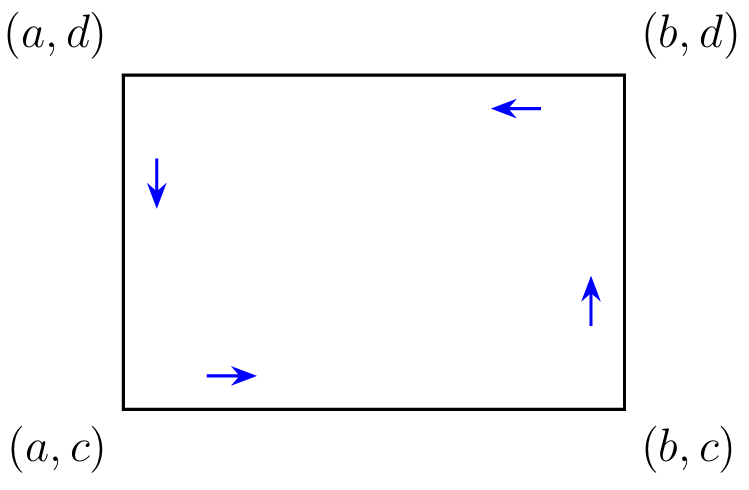
\includegraphics[width=0.5\textwidth]{figure/1.png}
\end{figure}

We say a function is holomorphic in $\overline R$ if there's an open neighborhood of U, $\overline R\subseteq U$ s.t. $f$ is holomorphic in U.

\section{Goursat Theorem}
\label{Goursat Theorem}
Let R be an rectangle and $f$ be a holomorphic function in $\overline R$, then $$\int_{\partial R}f\text dz=0$$
\subsection*{Proof}
For a rectangle R, define $$\eta(R):=\int_{\partial R}f\text dz$$
Divide R into four congruent rectangles $R^{(1)},R^{(2)},R^{(3)},R^{(4)}$, then 
$$\eta(R)=\eta(R^{(1)})+\eta(R^{(2)})+\eta(R^{(3)})+\eta(R^{(4)})$$
\begin{figure}[h]
    \centering
    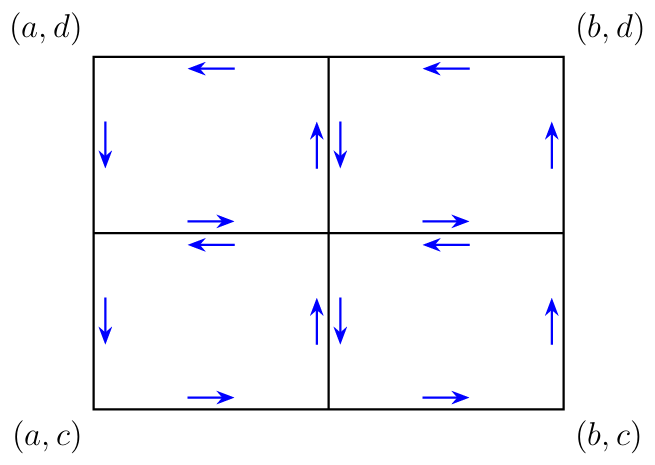
\includegraphics[width=0.5\textwidth]{figure/2.png}
\end{figure}

At most one small rectangle $R^{(k)}$ satisfies $$\abs{\eta(R^{(k)})}\geq \frac{1}4\abs{\eta(R)}$$
for some $1\leq k\leq 4$. We denote this rectangle by $R_1$. Continue this procession for $R_1$, we get a sub-rectangle $R_2\subseteq R_1$. By induction, we get sequence of nested rectangles $R_n$ s.t. $$\abs{\eta R(_n)}\geq 4^{-n}\abs{\eta(R)}$$
The rectangles $R_n\to z_0\in \overline R$

$\forall \epsilon>0$, choose $\delta>0$ s.t. $f$ is holomorphic in $D(z_0,\delta)$, and $\forall z\in D(z_0,\delta)$:
$$\abs{f(z)-f(z_0)-(z-z_0)f'(z_0)}\leq\epsilon\abs{z-z_0}$$

For $n$ large, $\overline {R_n}\subseteq D(z_0,\delta)$. By Corollary\ref{polynomial holomorphic}, we have
$$\int_{\partial {R_n}}\text dz=0$$
and $$\int_{\partial R_n}z\text dz=0$$
Hence
$$\begin{aligned}
    \abs{\eta(R_n)} &=\abs{\int_{\partial R_n}f(z)-f(z_0)-(z-z_0)f'(z_0)\text dz}\\
    &\leq \int_{\partial R_n}\abs{f(z)-f(z_0)-(z-z_0)f'(z_0)}\text dz\\
    &\leq \epsilon\int_{\partial R_n}\abs{z-z_0}\text ds\\
    &\leq \epsilon d_nL_n
\end{aligned}$$
where $d_n$ is the diameter of $R_n$, $L_n$ is the perimeter of $\partial R_n$. If $d$ is the diameter of R, and L is the perimeter of $\partial R$, then $$d_n=2^{-n}d\quad L_n=2^{-n}L$$
Hence we have
$$\abs{\eta(R_n)}\leq \epsilon 4^{-n}\text dL$$
By our assumption that $$\abs{\eta(R_n)}\geq 4^{-n}\abs{\eta(R)}$$
we have
$$\abs{\eta(R)}\leq \epsilon dL$$

Since $\epsilon$ is arbitrary, we have $\eta(R)=0$, which ends the proof.

\section{Cauchy's integral theorem on a disk}
Let $D\subseteq \mathbb C$ be a disk, $f:D\to \mathbb C$ a holomorphic function, $\gamma$ a closed rectifiable curve in D, then 
$$\int_\gamma f\text dz=0$$
\subsection*{Proof}
By theorem\ref{remark1}, it suffice to show there exists a function $F:D\to \mathbb C$, s.t. $$\fpart{F}{x}=f\quad \fpart{F}{y}=if$$

Without loss of generality we assume $D=\mathbb D$. Let $w=x+iy$, and  $\gamma_w$ be the piecewise linear curve $\gamma_w(0)= x$ and $\gamma_w(x) = x+iy$. Define
$$F(w):=\int_{\gamma_w}f\text dz$$
This implies $\fpart{F}{y}(w)=if(w)$. Actually, by the def of parital derivatives:
$$
\begin{aligned}
    \fpart{F}{y}(w) &:=\lim\limits_{\epsilon\to 0}\frac{F(w+\epsilon i)-F(w)}{\epsilon }\\
    &=\lim\limits_{\epsilon\to 0}\frac{\int_{\gamma_\epsilon}f\text dz}{\epsilon }\\
    &=if(w)
\end{aligned}
$$
where $\gamma_w$ is the linear curve $\gamma_w(x+iy)=x+iy+i\epsilon$. Let $\tilde {\gamma_w}$ be the piecewise linear curve that $\tilde {\gamma_w}(0)=iy$ and $\tilde {\gamma_w}(iy)=x+iy$. By theorem\ref{Goursat Theorem},we have $$F(w)=\int_{\tilde{\gamma_w}}f\text dz$$

This implies $\fpart{F}{x}(w)=f(w)$ by repeating the same argument for $\fpart{F}{y}(w)$, which finishes the proof.

(Note that the equality above is not a definition, it's actually equivalent to Goursat's theorem)

\chapter{Winding number}
Let $\gamma:[a,b]\to \mathbb C$ be a closed curve. Let $w\notin I_m\gamma$. 


Define $u:[a,b]\to S^1$$$U(t):=\frac{\gamma(t)-w}{\abs{\gamma(t)-w}}$$
Let $$\begin{aligned}
    \pi:&\mathbb R&\to& S^1\\ &s&\mapsto&e^{2\pi is}
\end{aligned}$$
$\Rightarrow$ $\exists$ lift of $u$, $$\tilde u:[a,b]\to \mathbb R$$continuous and $$\pi\circ \tilde u=u$$
such choice of $\tilde u$ is not unique, but if $\tilde u_1,\tilde u_2$ are two lift of $u$ $\Rightarrow$ $$\tilde u_1-\tilde u_2=l\in \mathbb Z$$
\section{Def}The winding number$$n(\gamma,w):=\tilde u(b)-\tilde u(a)$$
\section{prop}
\begin{itemize}
    \item[1] $n(\gamma,w)\in \mathbb Z$
    \item[2] $n(\gamma,w)$ take the same value when $w$ in a connected comp of $\mathbb C\setminus I_m\gamma$
    \item[3] Let $\Omega_\infty$ be the unbounded component of $\mathbb C\setminus Im\gamma$
\end{itemize}
\subsection*{Proof}
\subsubsection{1}Since $\gamma$ closed $\Rightarrow$$$e^{i2\pi\tilde u(b)}=e^{i2\pi\tilde u(a)}$$
$\Rightarrow$ $$\tilde u(b)-\tilde u(a)\in \mathbb Z$$
\subsubsection{2}
For a fixed $\gamma$ $n(\gamma,\cdot)$ is a continuous function w.r.t. $w$. SSince $\Omega$ connected, $$n(\gamma,\cdot):\Omega\to \mathbb Z$$the image $n(\gamma,\cdot)$ is connected in $\mathbb Z$, which implies single point, so $n(\gamma,\cdot)$ is a constant mapping.
\subsubsection{3}For $w\in \Omega_\infty$ $n(\gamma,\cdot)\to 0$ when $w\to \infty$, but $n(\gamma,w)\in \mathbb Z$ so $$n(\gamma,\cdot)=0\ \forall w\in \Omega_\infty$$
\section{Corollary}
$\mathbb D^*:=\mathbb D\setminus\{0\}$ is not simply connected.
\section{Prop}
(Winding number is homotopy invariant)
Given two closed curves.
$$\gamma_0:[a,b]\to\mathbb C\quad\gamma_1[a,b]\to\mathbb C$$
$H:[a,b]\times[0,1]\to \mathbb C\setminus\{w\}$ be a homotopy. Then$$n(\gamma_0,w)=n(\gamma_1,w)$$
\subsection*{Proof}Let $U:[a,b]\times[0,1]\to S^1$$$U(t,s):=\frac{H(t,s)-w}{\abs{H(t,s)-w}}$$
Then $\exists$ $\tilde U:[a,b]\times[0,1]\to \mathbb R$ continuous s.t.$$\pi\circ\tilde U=U$$where$\pi:\mathbb R\to S^1$ is the universal cover. Then $\forall s\in [0,1]$$$n(\gamma_s,w)=\tilde U(b,s)-\tilde U(a,s)$$
Since $\tilde U$ is continuous, $n(\gamma_s,w)\in \mathbb Z$, so $n(\gamma_s,w)$ is a constant $\forall s\in [0,1]$$\Rightarrow$$$n(\gamma_0,w)=n(\gamma_1,w)$$
\section{Lemma: Winding number formula for rectifiable curves}
$\gamma:[a,b]\to \mathbb C$ rectifiable, closed curve, let $w\notin Im\gamma$$$n(\gamma,w)=\frac{1}{2\pi i}\int_\gamma\frac{1}{z-w}\text dz$$
\subsection*{Proof}
Assume $\gamma$ is piecewise smooth. Consider $h:[a,b]\to\mathbb C$$$h(t):=\frac{1}{2\pi i}\int_a^t\frac{\gamma'(s)}{\gamma(s)-w}\text ds$$ $h$ piecewise smooth.$$h'(t)=\frac{1}{2\pi i}\frac{\gamma'(t)}{\gamma(t)-w}$$
and $$\left(e^{-2\pi ih(t)}(\gamma(t)-w)\right)'=0$$ outside a finite set. So$$e^{2\pi ih(t)}=\frac{\gamma(t)-w}{\gamma(a)-w}\quad\forall t\in [a,b]$$
On the other hand, $\tilde u:[a,b]\to\mathbb R$$$e^{2\pi i\tilde u(t)}=\frac{\gamma(t)-w}{\abs{\gamma(a)-w}}$$
Let $v(t):=\ln\abs{\gamma(t)-w}$, then we have:
$$e^{2\pi i\tilde u(t)+v(t)}=\gamma(t)-w$$$\Rightarrow$$\exists$ constant $\alpha\in \mathbb C$ s.t.$$2\pi i h(t)=2\pi i\tilde u(t)+\alpha$$then we have$$n(\gamma,w):=\tilde u(b)-\tilde u(a)=h(b)-h(a)$$
\section{Jordan Curve Theorem}
$\gamma$ a closed curve, $\gamma$ is simple(no self crossing: if $\forall t\neq s\in (a,b)$, have $\gamma(t)\neq \gamma(s)$)

Let $\gamma$ a simple closed curve. Then $\mathbb C\setminus Im\gamma$ has two connected components.


\chapter{Cauchy's integral formula}
\section{Lemma}
(A generalization of Gousat's theorem)
Let $R$ be an rectangle, and let $E\subseteq R$ be a finite set, let U be an open set s.t. $\overline R\subseteq U$ let $f:U\setminus E\to \mathbb C$ holomorphic, moreover$$\lim\limits_{z\to \xi}(z-\xi)f(z)=0\ \forall \xi\in E$$ then$$\in_{\partial R}f\text dz=0$$
\subsection{Proof}
We can decompose R into small rectangles s.t small rectangle contains one pt in E, We can assume $E=\{\xi\}$ $\forall \epsilon>0$, we can decompose R into 9 rectangle s.t. in the center rectangle $R_0$$$\abs{f(z)}\leq\frac{\epsilon}{\abs{z-\xi}}\quad\forall z\in \partial R_0$$ 
\begin{figure}
    \centering
    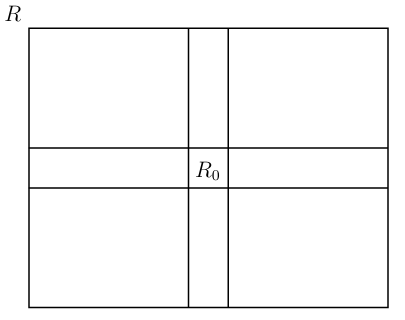
\includegraphics[width=0.5\textwidth]{figure/3.png}
\end{figure}
By original Gousat's theorem$$\int_{\partial R}f\text dz=\int_{\partial R_0}f\text dz$$
Hence$$\abs{\int_{\partial R}f\text dz}\leq\epsilon\int_{\partial R_0}\frac{1}{\abs{z-\xi}}\text dz\leq 8\epsilon$$
Since $\epsilon$ can be arbitrarily small$$\int_{\partial R}f\text dz=0$$
\section{Corollary}
Let $D\subseteq\mathbb C$ disk let $E\subseteq D$ a finite set. Let $f:D\to \mathbb C$ continuous holomorphic in $D\setminus E$ moreover$$\lim\limits_{z\to \xi}(z-\xi)f(z)=0\quad\forall \xi \in E$$
Let $\gamma $ be a closed rectifiable curve in D, then $$\int_\gamma f\text dz=0$$
\section{Cauchy integral formula on a disk}
\label{Cauchy's integral formula on a disk}
Let $D\subseteq \mathbb C$ disk. Let $f:D\to \mathbb C$ holomorphic let $a\in D$, let $\gamma$ be a closed rectifiable curve s.t. $a\notin Im\gamma$, Then $$n(\gamma,a)f(a)=\frac{1}{2\pi i}\int_\gamma\frac{f(z)}{z-a}\text dz$$
\subsection*{Proof}
Define function $g:D\setminus\{a\}\to \mathbb C$$$g(z):=\frac{f(z)-f(a)}{z-a}$$\\
$g$ is holomorphic on $D\setminus\{a\}$, $g$ can be continuously extend to D.

Then by the previous Corollary, since $$\lim\limits_{z\to a}(z-a)g(z):=\lim\limits_{z\to a}f(z)-f(a)=0$$then$$\int_\gamma g(z)\text da=0$$
This implies$$n(\gamma,a)f(a):=\frac{1}{2\pi i}\int_\gamma\frac{f(a)}{z-a}\text dz\stackrel{\text{coro}}{=}\frac{f(z)}{z-a}\text dz$$
\section{Corollary}
\label{Corollary 4.4}
Let $D\subseteq \mathbb C$ disk. Let $f:\overline D\to \mathbb C$ be a holomorphic functions. Then $$f(z)=\frac{1}{2\pi i}\int_{\partial D}\frac{f(w)}{w-z}\text dw\quad\forall z\in D$$
\subsection*{Proof}
$\forall z\in D$, we have $n(\partial D,z)=1$. Let $D'$ be a slightly larger disk with the same center, $\overline D\subseteq D$, s.t. $f$ is holomorphic in $D'$. Apply Theorem\ref{Cauchy's integral formula on a disk}, and end the proof.
\section{Theorem}Holomorphic functions is locally a power series, in particular, it's $C^\infty$
\section{Theorem}
\label{Theorem 4.5}
Let $\gamma$ be a rectifiable curve, $\phi:Im\gamma\to \mathbb C$ continuous. For $z\notin Im \gamma$, define $$f(z):=\int_\gamma\frac{\phi(w)}{w-z}\text dw$$
Then $\forall z_0\in \mathbb C\setminus Im\gamma$ let $\gamma:=dist(z_0,Im\gamma)$ $f$ is a power series on $D(z_0,r)$
$$f(z)=\sum\limits_{n=0}^\infty\left(\int_\gamma\frac{\phi(w)}{(w-z_0)^{n}}\text dw\right)(z-z_0)^n$$
In particular, $f$ is holomorphic.
\subsection*{Proof}
Fix $z_0$,$w\in Im\gamma$, consider function $\frac{\phi(w)}{w-z}$ (as func of $z$). It has a power series expansion on $D(z_0,r)$
$$\frac{\phi(w)}{w-z}=\sum\limits_{n=0}^\infty\frac{\phi(w)}{(w-z_0)^n}(z-z_0)^n$$
The above formula holds for every $w\in Im\gamma$ and $z\in D(z_0,r)$ Define $g_n:Im\gamma\to \mathbb C$(function of w)
$$g_n(w):=\sum\limits_{k=0}^n\frac{\phi(w)}{(w-z_0)^{n+1}}(z-z_0)^{k}$$
We are going to show $g_n$ converges uniformly to $\frac{\phi(w)}{w-z}$ on $Im\gamma$. Let $M:=\max\limits_{w\in Im\gamma}\abs{\phi(w)}$ and $r':=\abs{z-z_0}<r$
$$\begin{aligned}
    \abs{g_n(w)-\frac{\phi(w)}{w-z}}&=\abs{\sum\limits_{k=n}^\infty\frac{\phi(w)}{(w-z_0)^{k+1}}(z-z_0)^k}\\
    &\leq M\sum\limits_{k=n}^\infty\abs{\frac{(z-z_0)^k}{(w-z_0)^{k+1}}}\\
    &\leq M\sum\limits_{k=n+1}^\infty(\frac{r'}r)^k\frac{1}{r'}
\end{aligned}$$

Then we have 
$$\begin{aligned}
    \int_\gamma\frac{\phi(w)}{w-z}&=\lim\limits_{n\to+\infty}\int_\gamma\frac{\phi(w)}{(w-z_0)^n}\text dw\\
    &=\lim\limits_{n\to\infty}\left(\int_\gamma\frac{\phi(w)}{(w-z_0)^n}\text dw(z-z_0)^n\right)\\
    &=\sum\limits_{k=0}^\infty(\int_\gamma\frac{\phi(w)}{(w-z_0)^n}\text dw)(z-z_0)^n
\end{aligned}$$

For function in $\mathbb R$, differentiable does not imply infinitely differentiable, but in $\mathbb C$:
\section{Corollary}
Let $D\subseteq \mathbb C$ be a disk. Let $f:\overline D\to \mathbb C$ be a holomorphic function. Then $f$ is equal to a power series on D.
\subsection*{Proof}
By Corollary\ref{Corollary 4.4}, we have$$f(z)=\frac{1}{2\pi i}\int_{\partial D}\frac{f(w)}{w-z}\text dw$$
Apply Theorem\ref{Theorem 4.5} and get the result.
\section{Morera Theorem}
Let $U\subseteq \mathbb C$ be an open set. Let $f:U\to \mathbb C$ be a continuous function. Assume for every closed rectifiable curve $\gamma$ in U, we have $$\int_\gamma f\text dz=0$$Then $f$ is holomorphic in U.
\subsection*{Proof}\label{locally power series}
(Holomorphic function is locally a power series)

If suffice to show the result on each connected component of U. So we can assume Y is connected. Fix $z_0\in U$, $\forall z\in U$, let $\gamma_z$ be any rectifiable curve connecting $z_0$ and $z$, define $$F(z):=\int_{\gamma_z}f\text dz$$
This def is independent of the choice of $\gamma_z$ be our assumption that $$\int_\gamma f\text dz=0$$
We have $F'=f$, which is holomorphic in U. Since $f$ is the derivative of a holomorphic function, by Corollary\ref{locally power series}, $f$ is holomorphic in U.
\section{Formula for higher derivatives}
\label{Formulae for higher derivatives}
Let $D:=D(z_0,r)\subseteq \mathbb C$ be a disk. Let $f:\overline D\to \mathbb C$ be a holomorphic function. Then the $n$-th derivative at $z_0$ satisfies
$$f^{(n)}(z_0)=\frac{n!}{2\pi i}\int_{\partial D}\frac{f(w)}{(w-z_0)^{n+1}}\text dw$$
\subsection*{Proof}
Apply Theorem\ref{Theorem 4.5} to the formula:
$$f(z)=\frac{1}{2\pi i}\int_{\partial D}\frac{f(w)}{w-z_0}\text dw$$
we get
$$f(z)=\sum\limits_{n=0}^\infty\left(\int_{\partial D}\frac{f(w)}{(w-z_0)^n}\text dw\right)(z-z_0)^n$$
By Tayler expansion:
$$f(z)=\sum\limits_{n=0}^\infty\frac{f^{(n)}(z_0)}{n!}(z-z_0)^n$$
We get the result by comparing the coefficient.
\section{Cauchy's estimate}
\label{Cauchy's estimate}
Let $D:=D(z_0,r)\subseteq \mathbb C$ be a disk. Let $f:\overline D\to \mathbb C$ be a holomorphic function. Let $$M:=\max_{z\in \partial D}\abs{f(z)}$$then
$$\abs{f^{(n)}}\leq Mn!r^{-n}$$
\subsection*{Proof}
By Theorem\ref{Formulae for higher derivatives}
$$
\begin{aligned}
    \abs{f^{(n)}(z_0)}&=\abs{\frac{n!}{2\pi i}\int_{\partial D}\frac{f(w)}{(w-z_0)^{n+1}}\text dw}\\
    &\leq\abs{\frac{n!}{2\pi i}\int_{\partial D}Mr^{-(n+1)}\text ds}\\
    &=Mn!r^{-n}
\end{aligned}
$$
\section{Liouvile's theorem}
\label{Liouville's theorem}
Let $f:\mathbb C\to \mathbb C$ be bounded holomorphic function. Then $f$ is a constant.
\subsection*{Proof}
Assume $\abs{f(z)}\leq M$ on $\mathbb C$. Let $R>0$ and $z_0\in \mathbb C$. Aplly Theorem\ref{Cauchy's estimate} to $D(z_0,R)$, we get $$\abs{f'(z_0)}\leq MR^{-1}$$
Let $R\to +\infty$ we get $f'(z_0)=0$ for every $z_0\in \mathbb C$ This implies $f$ is a constant, by the fundamental theorem of calculus.
\section{Fundamental Theorem of Algebra}
Let $f$ be a polynomial with complex coefficient, $\deg f\geq 1$. Then $f$ has at least one root in  $\mathbb C$.
\subsection*{Proof}
Assume by contradiction that $f$ has no roots in $\mathbb C$. Then $g:=\frac{1}{f}:\mathbb C\to \mathbb C$ is a holomorphic function. Since $\deg f\geq 1$, $$\abs{f(z)}\to +\infty\quad \abs{z}\to \infty$$
This implies $g$ is a bounded holomorphic function. By theorem\ref{Liouville's theorem}, $g$ is a constant, which implies $f$ is a constant, contradiction.
\section{Theorem}
(Local uniform limit of holomorphic functions is holomorphic)

Let $U\subseteq \mathbb C$ be an open set. Let $f_n:U\to \mathbb C$ be a sequence of holomorphic functions, converges uniformly to a function $f$ on any compact subset $K\subseteq U$. Then $f$ is holomorphic in U.
\subsection*{Proof}
Let D be a disk s.t. $\overline D\subseteq U$. By Cauchy integral formula\ref{Corollary 4.4}, we have $\forall z\in D$
$$f_n(z)=\frac{1}{2\pi i}\int_{\partial D}\frac{f_n(w)}{w-z}\text dw$$
Since $f_n\to f$ uniformly on $\overline D$, we have
$$f(z)=\frac{1}{2\pi i}\int_{\partial D}\frac{f(w)}{w-z}\text dw$$
This implies $f$ holomorphic in D, by Theorem\ref{Theorem 4.5}
\end{document}